\documentclass{article}
\usepackage{tcolorbox}
\usepackage{xcolor}


% Language setting
% Replace `english' with e.g. `spanish' to change the document language
\usepackage[english]{babel}

% Set page size and margins
% Replace `letterpaper' with `a4paper' for UK/EU standard size
\usepackage[letterpaper,top=2cm,bottom=2cm,left=3cm,right=3cm,marginparwidth=1.75cm]{geometry}

% Useful packages
\usepackage{amsmath}
\usepackage{graphicx}
\usepackage{amssymb}
\usepackage{bm}
\usepackage[colorlinks=true, allcolors=blue]{hyperref}

\title{Notes for CS 473: Fundamentals of Machine Learning}
\author{Chris Kong}

\begin{document}
\maketitle

\tableofcontents
\newpage


\section{Feasibility of Learning}
\subsection{Hoeffding Inequality}
To describe the boundaries of the outcome of a sample drawn from the population, we have the following inequality:
\begin{tcolorbox}[colback=yellow!20, colframe=yellow!90, title=Hoeffding Inequality, coltitle=black]
$\mathbb{P}[\mid \nu-\mu \mid > \epsilon] \leq 2e^{-2\epsilon^{2}N}$
\end{tcolorbox}
This is called \textbf{Hoeffding Inequality}. Note that in the inequality, $N$ represents the sample size; $\epsilon$ represents the closeness of approximation; $\nu$ represents the probability in the sample; $\mu$ represents the real probability in the population. 

\subsection{Boundaries in Learning}
How is the above inequality connected to the process of learning? Here is the answer. First let's re-examine the process:
\begin{itemize}
    \item $\mu$: Suppose for $\mu$, it means $h(x) \neq f(x)$ in the scale of population.
    \item $\nu$: Suppose for $\nu$, it means $h(x) \neq f(x)$ in the scale of sample.
\end{itemize}
Then we have it in a math form: 
\begin{align*}
    \mu &= \mathbb{P}[h(x) \neq f(x)] \equiv E_{out}(h) & \text{(Out-Sample Error)}\\
    \nu &= \frac{1}{N}\sum_{i=1}^{N}[h(x_{i}) \neq f(x_{i})] \equiv E_{in}(h) & \text{(In-Sample Error)}
\end{align*}
Then we can combine them with the \textbf{Hoeffding Inequality} and get the following:
\begin{tcolorbox}[colback=yellow!20, colframe=yellow!90, title=Expanded Hoeffding Inequality 1, coltitle=black]
$\mathbb{P}[\mid E_{in}(h) - E_{out}(h) \mid > \epsilon] \leq 2e^{-2\epsilon^{2}N}$
\end{tcolorbox}
However, this is not ideal for "Learning" and here is why:
\begin{itemize}
    \item This is only for a single hypothesis.
    \item What we have is a hypothesis space $\mathcal{H}$.
    \item With a single hypothesis, this is more like "testing" than "learning".
    \item We need to come up on $g \in \mathcal{H}$ which by definition is obtained after seeing the data.
\end{itemize}
Thus we want to move a bit further by estimating the function $g \in \{ h_{1}, h_{2}, ..., h_{m}\} = \mathcal{H}$:
\begin{align*}
    \mathbb{P}[\mid E_{in}(g) - E_{out}(g) \mid > \epsilon] & \leq \sum_{m=1}^{M} \mathbb{P}[\mid E_{in}(h_{m}) - E_{out}(h_{m}) \mid > \epsilon]\\
    & \leq \sum_{m=1}^{M}2e^{-2\epsilon^{2}N}\\
    \mathbb{P}[\mid E_{in}(g) - E_{out}(g) \mid > \epsilon] & \leq 2Me^{-2\epsilon^{2}N}
\end{align*}
In the above inequality, $M$(the number of hypothesis in $\mathcal{H}$) can be seen as the complexity of hypothesis space. Under certain assumptions (unseen samples are drawn with the same probability distribution P as the seen examples) we can bound the difference between in-sample and out-of-sample errors.
\begin{tcolorbox}[colback=yellow!20, colframe=yellow!90, title=Expanded Hoeffding Inequality 2, coltitle=black]
$\mathbb{P}[\mid E_{in}(g) - E_{out}(g) \mid > \epsilon] \leq 2Me^{-2\epsilon^{2}N}$
\end{tcolorbox}


\subsection{Summary and Thoughts}
\subsubsection{Summary}
\begin{itemize}
    \item The goal of learning is to approximate the behavior of the unknown function $f$.
    \item We are usually provided with a finite set of examples which respect the behavior of $f$ (which we usually call it Training Set).
    \item The assumption is that each example is independently drawn from drawn from the entire sample set with some probability distribution $\mathbf{P}$.
    \item We identify a hypothesis set $\mathcal{H}$ from which our goal is to pick a function $g$.
    \item $g$ should be such that it approximates the function f on unseen data.
    \item The inequality implies that if we can bring the in-sample error towards zero we can probabilistically guarantee that out-of-sample error will not be far either. This essentially means that the hypothesis $g$ will probabilistically approximate function $f$.
\end{itemize}
Here are two key questions:
\begin{enumerate}
    \item Can we make sure that $E_{out}(g)$ is close to $E_{in}(g)$?
    \item Can we make $E_{in}(g)$ small enough?
\end{enumerate}
Hoeffding Inequality only addresses the first question. The second question is addressed by actually choosing a hypothesis set, running the learning algorithm and seeing how low can we make $E_{in}(g)$.

\subsubsection{Complexity of $\mathcal{H}$}
\begin{itemize}
    \item There is a trade-off in deciding how complex should the hypothesis space ($M$) be.
    \item More complex hypothesis enables us to choose a complex $g$ which increases the chances of making $E_{in}(g) \approx 0$.
    \item At the same time a complex hypothesis space makes the above bound loose making the gap between $E_{in}(g)$ and $E_{out}(g)$ large.
\end{itemize}

\subsubsection{Complexity of $f$}
\begin{itemize}
    \item Complexity of $f$ impacts the second question above.
    \item A more complex $f$ is harder to learn and hence will require a more complex $g$ which in-turn implies a more complex hypothesis set $\mathcal{H}$.
\end{itemize}
\newpage

\section{Linear Models for Regression}
\subsection{Loss Function as Error Measure}
As the hypothesis $h$ approaches the unknown function $f$, we would like to have a function to measure its error, such as $E(h,f)$. Even through the sample space $\mathcal{X}$ could be continuous in practical scenario, we define a point-wise error measure as below:
\begin{tcolorbox}[colback=yellow!20, colframe=yellow!90, title=Basic Error Measure Function, coltitle=black]
$E(h,f) = \sum_{i=1}^{N}e(h(x_{i}), f(x_{i}))^{2}$
\end{tcolorbox}
The function $e(h,f)$ here can have multiple connotations when measuring different kind of errors, and here are some examples:
\begin{itemize}
    \item Binary classification error: $e(h, f)=[h(x)\neq f(x)]$
    \item Squared error: $e(h,f)=(h(x)-f(x))^{2}$
    \item Cross-entropy loss: $-[y\log p + (1-y)\log (1-p)]$
\end{itemize}
\subsection{Linear Regression}
The basic linear regression takes form:
\begin{align*}
    g(X) = \beta_{0} + \sum_{i=1}^{p}\beta_{i}x_{i}
\end{align*}
The learnable parameters are $\beta = (\beta_{1}, \beta_{2}, ..., \beta_{p})$. The model assumes that either the unknown function $f$ is linear or it can be approximated well as a linear function.\\
Note that even though it is a linear function, the input variables $\mathbf{x}$ could take various forms. For example:
\begin{itemize}
    \item Original inputs: $x_{1}, ..., x_{p}$
    \item Transformations of inputs: $\log(x_1), ... \log(x_{i})$
    \item Basis expansions: $x_{i+1} = x_{1}^{2}; x_{i+2} = x_{1}^{3}$ etc
    \item Composition of different variables: $x_{i+1} = x_{1} \cdot x_{2}$ etc
\end{itemize}

\subsection{Linear Regression Model: Training}
We have a set of examples as training data: $D = {(x^{1}, y^{1}), (x^{1}, y^{1}), ..., (x^{N}, y^{N})}$, where $x^{i} = [x_{1}^{i}, x_{2}^{i}, ..., x_{p}^{i}]$.\\

To learn the parameter, we define an error metric (a loss function) which measures the discrepancy between the model prediction and the actual value on the training set. One reasonable metric is the squared error between the two quantities:
\begin{align*}
    Loss(\beta) = RSS(\beta) &= \sum_{i=1}^{N}(y^{i}-g_{\beta}(x^{i}))^{2}\\
    &= \sum_{i=1}^{N}(y^{i}-(\beta_{0} + \sum_{j=1}^{p}\beta_{j}x_{j}^{i}))^{2}\\
    &= \sum_{i=1}^{N}(y^{i}-\beta_{0} - \sum_{j=1}^{p}\beta_{j}x_{j}^{i})^{2}
\end{align*}
Note that the "RSS" here means "Residual Sum of Squares" and the meaning of "Learning": to adjust the parameters $\beta = [\beta_{0}, \beta_{1}, ..., \beta_{p}]$. Now let us re-examine the "complex" equation and try to rewrite it using linear algebra. In this sense, we will have $\bm{\beta}^{T} = [\beta_{0}, \beta_{1}, ..., \beta{p}]$ and $\mathbf{X} = [1, x_{1}, x_{2}, ..., x_{p}]$. Thus we have:
\begin{align*}
    y = g_{\bm{\beta}}(\mathbf{X}) = \mathbf{X}\cdot \bm{\beta}
\end{align*}
Then we can have the Loss Function:
\begin{tcolorbox}[colback=yellow!20, colframe=yellow!90, title=Loss Function, coltitle=black]
    $Loss(\beta) = RSS(\beta) = \sum_{i=1}^{N}(y^{i}-\beta_{0} - \sum_{j=1}^{p}\beta_{j}x_{j}^{i})^{2} = (\bm{y}-\bm{X}\beta)^{T} \cdot (\bm{y}-\bm{X}\beta)$
\end{tcolorbox}
Remember this is a "loss" function, meaning that it measures the loss of our prediction against the actual values. Thus our goal now is to reduce or to minimize the loss to optimize our function. In other words, to minimize the loss is to find hypothesis function $g$ that approximates the true function $f$. To realize this, we need to find the derivative of RSS($\beta$) and set it to zero:
\begin{align*}
    \frac{\partial RSS}{\partial \beta} &= -2\bm{X}^{T}(\bm{y}-\bm{X}\beta) = 0\\
    \hat{\beta} &= (\bm{X}^{T} \bm{X})^{-1}\bm{X}^{T}\bm{y}
\end{align*}
And now we have a closed form solution! Now let's carry on to the next part: Prediction.

\subsection{Linear Regression Model: Prediction}
Simplify the equation by writing it in matrix form and augmenting the vector of inputs $\bm{x}$ by $1$ and subsuming the intercept/bias $\beta$ into the parameter vector $\bm{\beta}$: $\bm{\beta} = [\beta_{0}, \beta_{1}, ..., \beta_{p}]$ and $\bm{X} = [1, x_{1}, ..., x_{p}]$. Then we will have the following form:
\begin{align*}
    y = g_{\beta}(\bm{X}) = \bm{X} \cdot \bm{\beta}\\
    \hat{\bm{\beta}} = (\bm{X}^{T} \bm{X})^{-1}\bm{X}^{T}\bm{y}
\end{align*}
Now we can do the prediction. For a new observation $x_{0}$, its prediction can be computed as:
\begin{align*}
    \hat{y}_{0} &= [1,x_{0}] \cdot \hat{\beta}\\
    &= [1,x_{0}] \cdot (\bm{X}^{T} \bm{X})^{-1}\bm{X}^{T}\bm{y}
\end{align*}

\subsection{Shrinkage Methods (Regularization)}

Linear models as-is, particularly those with a large number of variables (and their compositions), trained using least squares estimates, have two flaws:
\begin{enumerate}
    \item They can tune well on the provided snapshot of the training data but may not have a low out-of-sample error. This is the Bias-Variance trade-off which we will talk about in detail later.
    \item A model with large number of variables is less suited for model interpretation. Typically we would like to know which (handful) variables have the most predictive power.
\end{enumerate}
In order to deal with the above flaws, we come up with several methods and "Regularization" is one of them. This is accomplished by augmenting the training of the models in a way so that minimizing the loss function leads to "shrinking"/"deleting" the effect of unimportant variables, which would be effective in preventing the problem of "over-fitting". Here are several ways of \textbf{subset selection}:
\begin{itemize}
    \item Forward and Backward-Stepwise Selection
    \item Forward-Stagewise Regression
    \item Skrinkage methods - Ridge and Lasso - Regularization
\end{itemize}
Here we will discuss Regularization: Ridge and Lasso Regression in particular.

\subsubsection{Ridge Regression}
For Ridge Regression, we impose a penalty on the size of the coefficients being learned:
\begin{align*}
    \hat{\beta}^{ridge} = argmin_{\beta}\sum_{i=1}^{N}\left(y^{i}-\beta_{0}-\sum_{j=1}^{p}x_{j}^{i} \cdot \beta_{j}\right)^{2}\\
    \text{subject to} \sum_{j=1}^{p}\beta_{j}^{2} \leq s
\end{align*}
Note that this is a $\bm{L}_{2}$ penalty or Weight Decay. The above can also be re-written as:
\begin{align*}
    \hat{\beta}^{ridge} = argmin_{\beta}\left[ \sum_{i=1}^{N}\left(y^{i}-\beta_{0}-\sum_{j=1}^{p}x_{j}^{i} \cdot \beta_{j}\right)^{2} + \lambda \sum_{j=1}^{p}\beta_{j}^{2}\right]
\end{align*}
This formula represents the objective of finding a set of parameters \( \beta \) (including \( \beta_0, \beta_1, \ldots, \beta_p \)) that minimizes the overall value of the expression.\\

\textbf{First Part: Residual Sum of Squares}
\[
\sum_{i=1}^{N}\left(y^{i}-\beta_{0}-\sum_{j=1}^{p}x_{j}^{i} \cdot \beta_{j}\right)^{2}
\]
This part calculates the squared difference between the model's predictions and the actual values, known as residuals. For each observation \( i \) (from 1 to \( N \)), the difference between the predicted and actual value \( y^{i} \) is squared. All these squared differences are then summed up. This is the part we aim to minimize as we want the model's predictions to be as close to the actual values as possible.\\

\textbf{Second Part: L2 Regularization Term}
\[
\lambda \sum_{j=1}^{p}\beta_{j}^{2}
\]
This part is the essence of Ridge Regression and what differentiates it from ordinary linear regression. It's a regularization term that penalizes the complexity of the model. Specifically, it penalizes the magnitude of the model parameters \( \beta_j \). The parameter \( \lambda \) is a hyper-parameter that adjusts the strength of regularization: as \( \lambda \) increases, the regularization strength increases, and the magnitude of the model parameters decreases. When \( \lambda = 0 \), Ridge Regression reduces to ordinary linear regression.\\

\textbf{Summary}
\begin{tcolorbox}[colback=yellow!20, colframe=yellow!90, title=Ridge Regression, coltitle=black]
$ \hat{\beta}^{ridge} = argmin_{\beta}\left[ \sum_{i=1}^{N}\left(y^{i}-\beta_{0}-\sum_{j=1}^{p}x_{j}^{i} \cdot \beta_{j}\right)^{2} + \lambda \sum_{j=1}^{p}\beta_{j}^{2}\right]$
\end{tcolorbox}
The objective of this formula is to find a set of parameters \( \beta \) that minimizes the squared difference between the model's predictions and the actual values while taking into account the complexity of the model. This is achieved by minimizing a combination of the residual sum of squares and the regularization term. In addition, we can find its matrix expression are written as follow:
\begin{align*}
    RSS(\lambda) &= \left(\bm{y} - \bm{X}\bm{\beta} \right)^{T} \left(\bm{y} - \bm{X}\bm{\beta} \right) + \lambda \bm{\beta}^{T}\bm{\beta}\\
    \hat{\beta}^{ridge} &= \left(\bm{X}^{T}\bm{X} + \lambda\bm{I} \right)^{-1}\bm{X}^{T}\bm{y}
\end{align*}

\subsubsection{Lasso Regression}
Lasso is similar to Ridge Regression but the penalty is different:
\begin{align*}
     \hat{\beta}^{lasso} = argmin_{\beta}\sum_{i=1}^{N}\left(y^{i}-\beta_{0}-\sum_{j=1}^{p}x_{j}^{i} \cdot \beta_{j}\right)^{2}\\
    \text{subject to} \sum_{j=1}^{p} \mid \beta_{j} \mid \leq t
\end{align*}
\begin{tcolorbox}[colback=yellow!20, colframe=yellow!90, title=Lasso Regression, coltitle=black]
$ \hat{\beta}^{lasso} = argmin_{\beta}\left[ \sum_{i=1}^{N}\left(y^{i}-\beta_{0}-\sum_{j=1}^{p}x_{j}^{i} \cdot \beta_{j}\right)^{2} + \lambda \sum_{j=1}^{p}\beta_{j}^{q}\right]$
\end{tcolorbox}

\subsubsection{Ridge Regression Review}

Ridge Regression adds an L2 regularization term to the loss function of linear regression. Its mathematical form is:
\[
J(\theta) = \frac{1}{2m} \sum_{i=1}^{m} (h_{\theta}(x^{(i)}) - y^{(i)})^2 + \lambda \sum_{j=1}^{n} \theta_j^2
\]
Where:
\begin{itemize}
    \item \( J(\theta) \) is the loss function.
    \item \( h_{\theta}(x^{(i)}) \) is the hypothesis function, typically \( h_{\theta}(x) = \theta^T x \).
    \item \( m \) is the number of training samples.
    \item \( \theta \) are the model parameters.
    \item \( \lambda \) is the regularization parameter.
    \item \( n \) is the number of features.
\end{itemize}

\subsubsection{Lasso Regression Review}

Lasso Regression adds an L1 regularization term to the loss function of linear regression. Its mathematical form is:
\[
J(\theta) = \frac{1}{2m} \sum_{i=1}^{m} (h_{\theta}(x^{(i)}) - y^{(i)})^2 + \lambda \sum_{j=1}^{n} |\theta_j|
\]
Similar to Ridge Regression, but the regularization term is the sum of the absolute values of the parameters.

\subsubsection{Comparison and Thoughts}

The main difference between the two lies in the regularization term:
\begin{itemize}
    \item Ridge Regression uses L2 regularization, which shrinks the magnitude of the coefficients but doesn't make them exactly zero.
    \item Lasso Regression uses L1 regularization, which can make some coefficients exactly zero, thus performing feature selection.
\end{itemize}
The choice between the two regularization methods depends on the specific application and data.
\newpage

\section{Over-fitting and Cross Validation}
\subsection{Over-fitting}
Over-fitting is fitting the data more than what we want. It is a phenomenon where fitting the data well no longer indicates that we will get a decent out-of-sample error. In fact, it may enlarge the out-of-sample error.

\subsection{Regularization}
Remember what we just learned about regularization and we have the following expression:
\begin{align*}
    min\left[ E_{in}(\bm{w}) + \frac{\lambda}{N} \bm{w}^{T}\bm{w} \right]
\end{align*}
The $\lambda$ here penalizes the parameters. The larger $\lambda$ is, the weaker the power of the fitting is. Intuitively enlarging the $\lambda$ will loosen the fitting line. A $\lambda$ that is too large will ultimately cause under-fitting.

\subsection{Validation and Cross Validation}
Before we dive deeper, we should know some basics, three components of data:
\begin{itemize}
    \item \textbf{Training Data: }the data you use to tune the parameters of the model (search for the hypothesis);
    \item \textbf{Validation Data: }part of the data you use to test the goodness of the running hypothesis. Performance on the validation set is a surrogate of the performance on unseen examples — so long as the validation set is drawn from the same distribution as the test set;
    \item \textbf{Test Data: }once you are happy with your chosen hypothesis, test data is used to measure the final performance of the model. There is no going back after this! Otherwise you will be cheating and all bets are off whether your model will generalize to unseen data.
\end{itemize}
The big assumption here is that the dataset is representative of the real world. Throughout the learning we track the performance on the validation set. Validation Data is also used to avoid over-fitting as the $E_{out}$ will be large given by the validation data.

\subsubsection{Validation}
For any hypothesis $h$, we have:
\begin{align*}
    E_{out}(h) = E_{in}(h) + \text{Penalty for over-fitting}
\end{align*}
Before the math for validation, let us first formalize it:
\begin{itemize}
    \item Dataset $\bm{D} = \{(x_1, y_1), (x_2, y_2), ..., (x_N, y_N) \}$
    \item Training set $\bm{D}_{train} \in D \leftarrow \bm{N} - \bm{K}$ examples
    \item Validation set $\bm{D}_{val} \in D \leftarrow \bm{K}$ examples
    \item Hypothesis $g^{-}$: the hypothesis selected after training the model on $\bm{D}_{train}$
\end{itemize}
Now we can write out the error function for the validation set:
\begin{align*}
    E_{val}(g^{-}) = \frac{1}{K} \sum_{x_{n}\in D_{val}} e\left( g^{-}(x_{n}), y_{n} \right) 
\end{align*}
But how is the Error of Validation of $g^-$ reasonable for estimating Out-of-sample Error of $g^-$? Let's have some maths here:

\begin{align*}
    \mathbb{E} \left[ E_{val}(g^{-}) \right]
    &= \mathbb{E}_{D_{val}} \left[ \frac{1}{K}\sum_{x_{n}\in D_{val}} e\left( g^{-}(x_{n}), y_{n} \right) \right]\\
    &= \frac{1}{K} \sum_{x_{n}\in D_{val}} \mathbb{E}_{D_{val}} \left[ e\left( g^{-}(x_{n}), y_{n} \right)\right]\\
    &= \frac{1}{K} \sum_{x_{n}\in D_{val}} E_{out}(g^{-})\\
    &= E_{out}(g^{-})
\end{align*}
Thus we have:
\begin{align*}
    \mathbb{E} \left[ E_{val}(g^{-}) \right]
    &= \frac{1}{K} \sum_{x_{n}\in D_{val}} \mathbb{E}_{D_{val}} \left[ e\left( g^{-}(x_{n}), y_{n} \right)\right]
    =  E_{out}(g^{-})\\
    \mathbb{V} \left[ E_{val}(g^{-}) \right]
    &= \frac{1}{K^{2}} \sum_{x_{n}\in D_{val}} \mathbb{V}_{D_{val}} \left[ e\left( g^{-}(x_{n}), y_{n} \right)\right]
    =  \frac{\sigma^{2}}{K}
\end{align*}
And we also have a key inequality:
\begin{align*}
     E_{out}(g^{-}) \leq  E_{val}(g^{-}) + O\left( \frac{1}{\sqrt{K}} \right)
\end{align*}
Then we can take a look at Model Selection process as follow:

\begin{figure}[h]
\centering
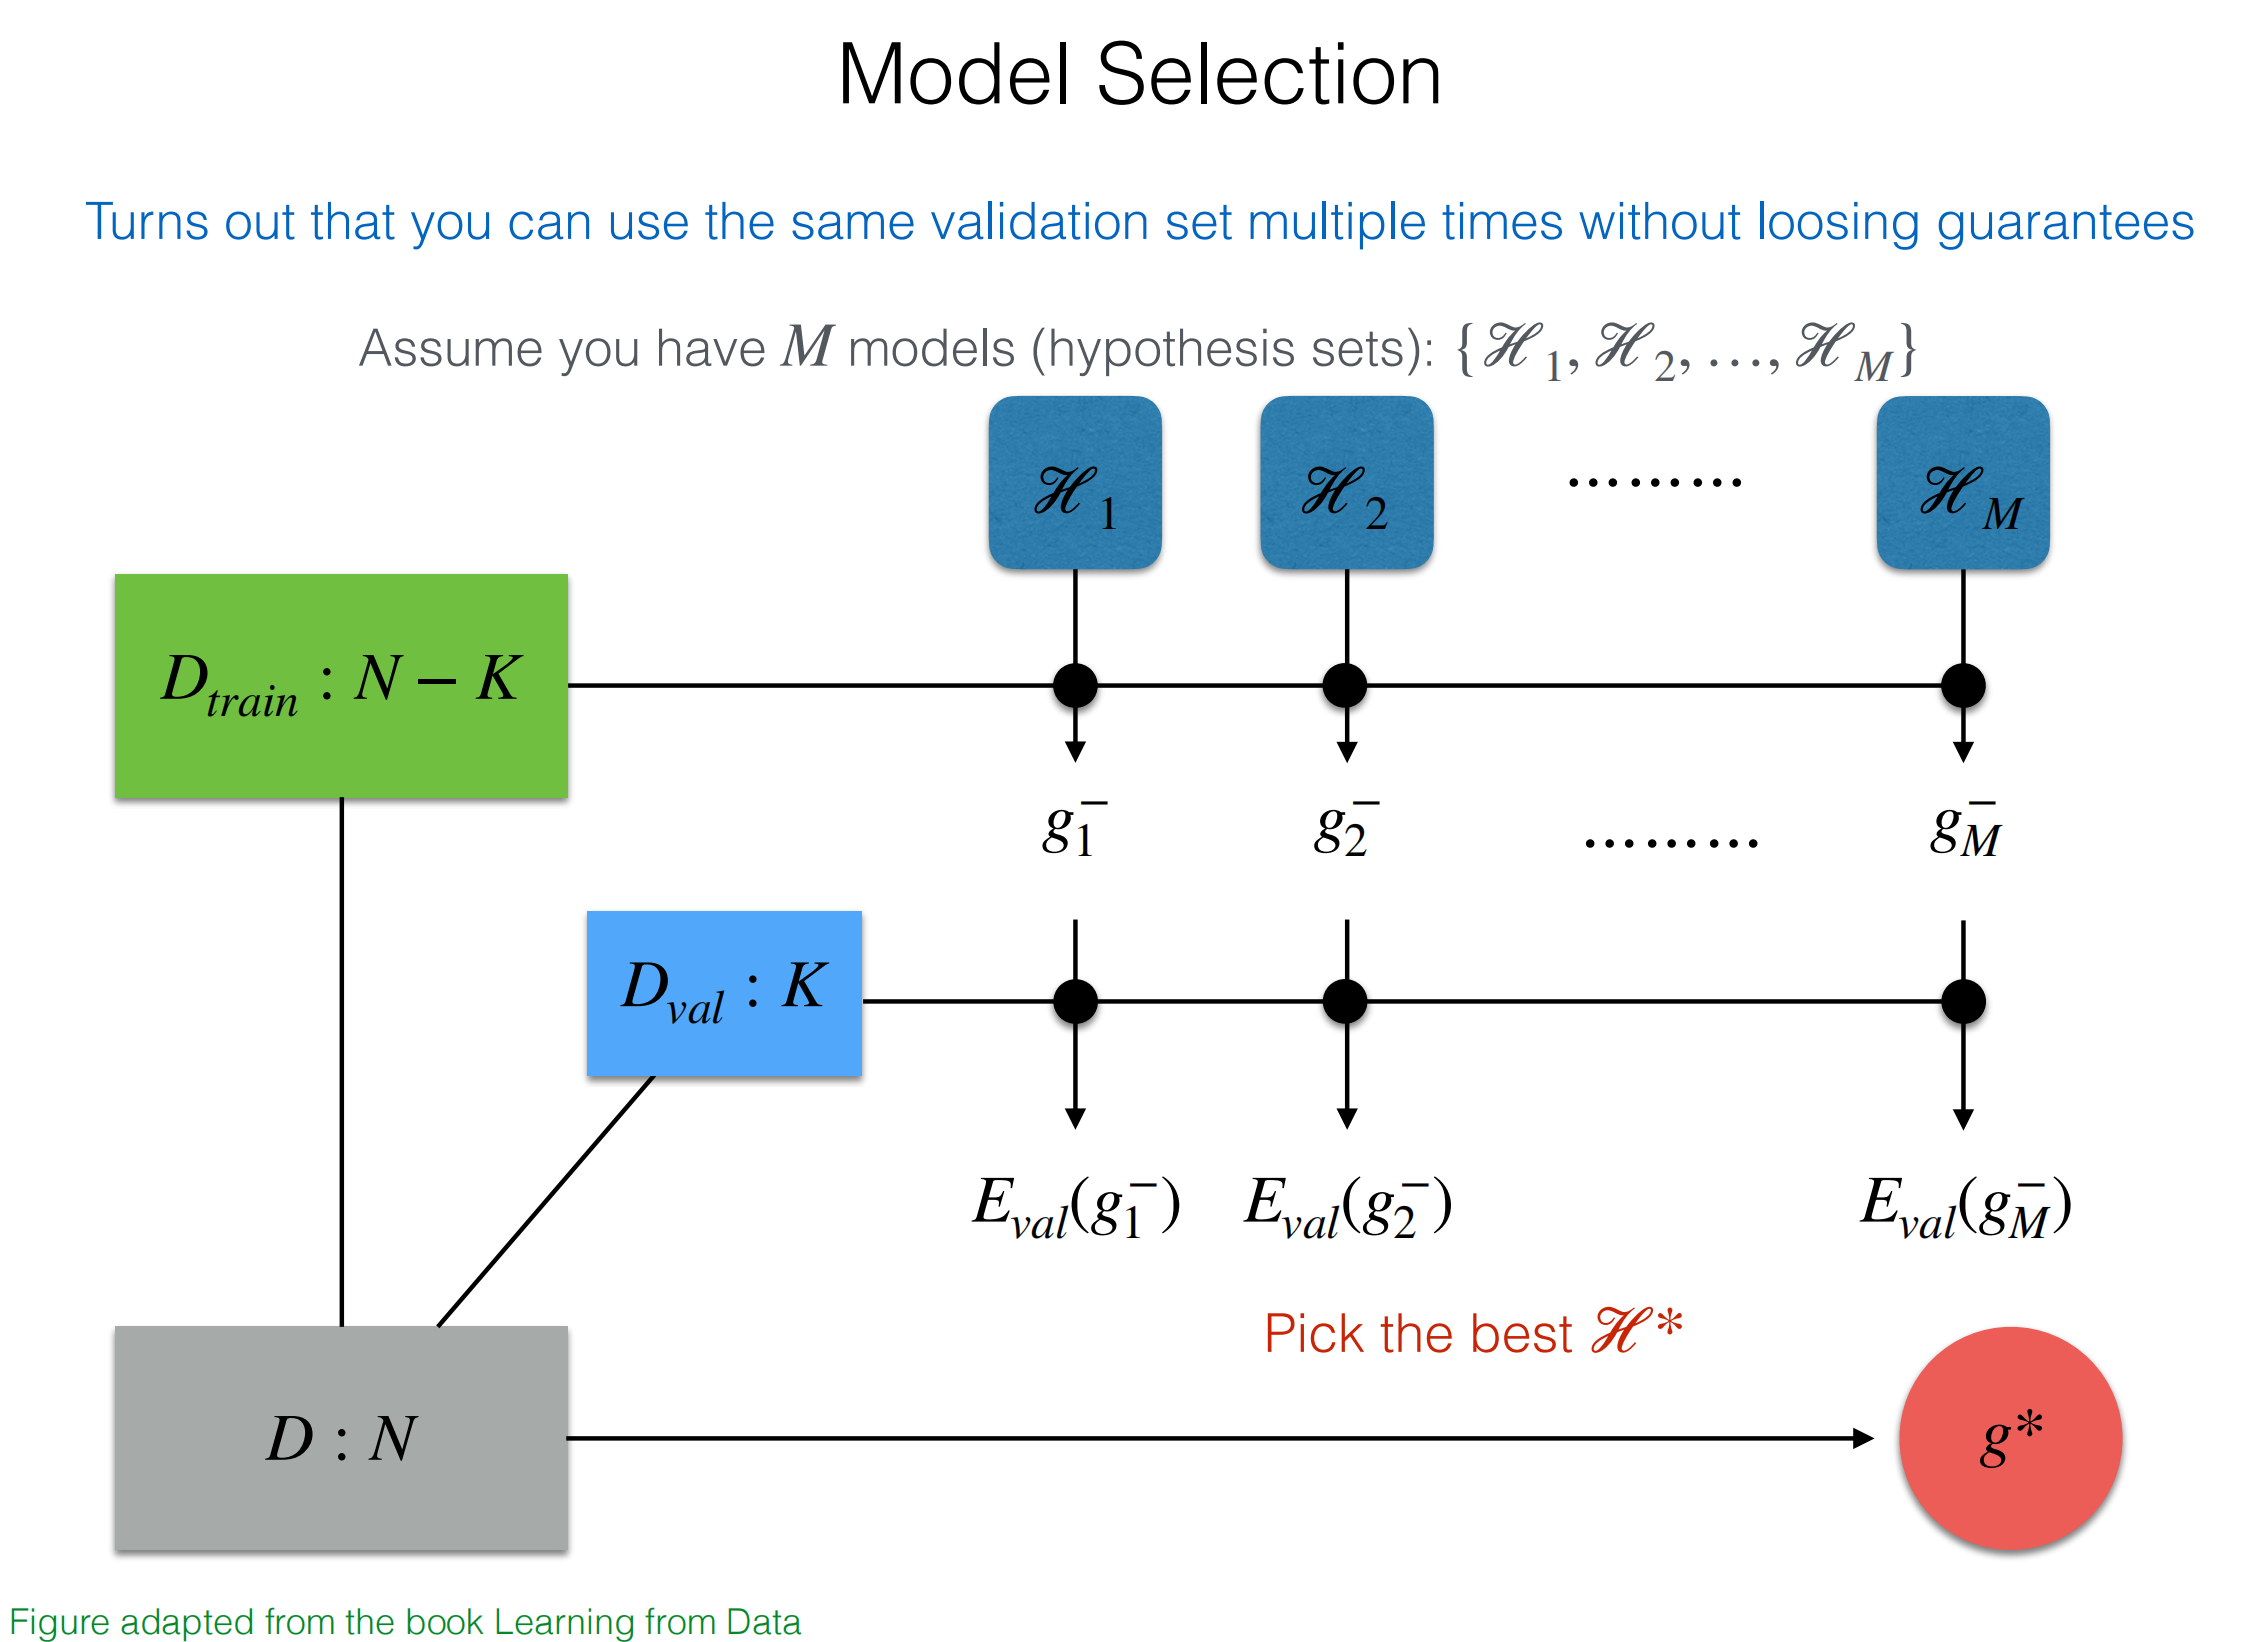
\includegraphics[width=16cm]{3.3.1_Model.png}
\end{figure}

\subsubsection{Cross Validation}
Cross Validation (CV) is a statistical method used to estimate the performance of machine learning models. It helps in understanding how the results of a statistical analysis will generalize to an independent dataset. Instead of using the entire dataset to both train and validate the model, it's split multiple times for both purposes. Here's a brief overview:

\begin{enumerate}
    \item \textbf{K-Fold CV}:
    \begin{itemize}
        \item The most commonly used method of cross-validation.
        \item The dataset is randomly partitioned into \( k \) equal-sized subsamples.
        \item Of the \( k \) subsamples, a single subsample is retained as the validation data for testing the model, and the remaining \( k-1 \) subsamples are used as training data.
        \item The cross-validation process is then repeated \( k \) times, with each of the \( k \) subsamples used exactly once as the validation data.
        \item The \( k \) results from the folds can then be averaged (or otherwise combined) to produce a single estimation.
    \end{itemize}

    \item \textbf{Stratified K-Fold CV}:
    \begin{itemize}
        \item Variation of K-Fold CV where each fold is made by preserving the percentage of samples for each class.
        \item Particularly useful for imbalanced datasets.
    \end{itemize}

    \item \textbf{Leave-One-Out CV (LOOCV)}:
    \begin{itemize}
        \item A special case of k-fold CV where \( k \) is set to the number of observations in the dataset.
        \item For a dataset with \( N \) observations, \( N \) separate times the learning algorithm is trained, each time leaving out one observation.
    \end{itemize}

    \item \textbf{Leave-P-Out CV}:
    \begin{itemize}
        \item Similar to LOOCV, but instead of leaving one observation out, we leave \( P \) observations out.
    \end{itemize}

    \item \textbf{Time-Series CV}:
    \begin{itemize}
        \item Variation for time-ordered data. Instead of randomly partitioning, it takes into account the order of the data.
    \end{itemize}
\end{enumerate}

\textbf{Advantages}:
\begin{itemize}
    \item Provides a more accurate estimate of out-of-sample accuracy.
    \item More "efficient" use of data as every observation is used for both training and validation.
\end{itemize}

\textbf{Disadvantages}:
\begin{itemize}
    \item Computationally expensive, especially for large datasets or complex models.
\end{itemize}

In essence, cross-validation provides a tool to predict the performance of a model on unseen data and helps in preventing overfitting.\\

\textbf{Model Selection with Cross Validation:}
\begin{enumerate}
    \item Define $M$ models by choosing different values of $\lambda: (\mathcal{H}, \lambda_{1}), (\mathcal{H}, \lambda_{2}), ..., (\mathcal{H}, \lambda_{M})$;
    \item Run the cross validation module to get an estimate of the cross validation error $E_{CV}(g^{m})$;
    \item Pick the model $(\mathcal{H}, \lambda^{*})$ with the smallest error;
    \item Train the model $(\mathcal{H}, \lambda^{*})$ on the entire training set $D$ to obtain the final hypothesis $g^{m^{*}}$.
\end{enumerate}

\subsection{Bias and Variance}
Before we go further, let us have a brief review:
\begin{itemize}
    \item $E_{out}$: out-of-sample error (unknown);
    \item $E_{in}$: in-sample error (training error - known);
    \item Complex $\mathcal{H}$: better chance of approximating $f$ in-sample (low training error);
    \item Simple $\mathcal{H}$: better chance of generalizing out-of-sample (low generalization error);
    \item Understand: the goal of Machine Learning is to lowing $E_{out}$ as much as possible given the observed dataset.
\end{itemize}

Bias-variance allows us to express $E_{out}$ in a way that provides some cues to what hypothesis space to start with. It tells you:
\begin{enumerate}
    \item How well $\mathcal{H}$ can approximate $f$;
    \item How well we can zoom in on a good hypothesis $h \in \mathcal{H}$.
\end{enumerate}
Note that BV analysis applies to only real-valued targets and uses squared error metric. Now let us start with some maths:
\begin{align*}
    \mathbb{E}_{D}\left[ E_{out}(g^{D}) \right]
    &= \mathbb{E}_{D} \left[ \mathbb{E}_{x} \left[  (g^{D}(x) - f(x))^{2} \right]  \right]\\
    &= \mathbb{E}_{x} \left[ \mathbb{E}_{D} \left[  (g^{D}(x) - f(x))^{2} \right]  \right]\\
    &= \mathbb{E}_{x} \left[ \mathbb{E}_{D} \left[  (g^{D}(x))^{2} \right] -2\mathbb{E}_{D}[g^{D}(x)]f(x) + f(x)^{2} \right]
\end{align*}
Assume that we will have multiple training datasets: $\{ D_1, D_2, ..., D_K \}$, then:
\begin{align*}
    \mathbb{E}_{D} \left[  (g^{D}(x))^{2} \right] \approx \frac{1}{K} \sum_{i=1}^{K} g^{D_{i}}(x) = \Bar{g}(x)
\end{align*}
Then we can rewrite our equation into the form that contains Variance and Bias:
\begin{align*}
    \mathbb{E}_{D}\left[ E_{out}(g^{D}) \right]
    &= \mathbb{E}_{x} \left[ \mathbb{E}_{D} \left[  (g^{D}(x))^{2} \right] -2\Bar{g}(x)f(x) + f(x)^{2} \right]\\
    &= \mathbb{E}_{x} \left[ \mathbb{E}_{D} \left[  (g^{D}(x))^{2} \right]-\Bar{y}(g)^{2}+\Bar{y}(g)^{2} -2\Bar{g}(x)f(x) + f(x)^{2} \right]\\
    &= \mathbb{E}_{x} \left[ \mathbb{E}_{D} \left[  (g^{D}(x))^{2} -\Bar{y}(g)^{2}\right]+\left[  \Bar{y}(g) - f(x)\right]^{2} \right]
\end{align*}
From the above equation, we now have:
\begin{align*}
    \textbf{var} &= \mathbb{E}_{D} \left[  (g^{D}(x))^{2} -\Bar{y}(g)^{2}\right]\\
    \textbf{bias} &= \left[  \Bar{y}(g) - f(x)\right]^{2}
\end{align*}
In conclusion:
\begin{align*}
     \mathbb{E}_{D}\left[ E_{out}(g^{D}) \right]
     &= \mathbb{E}_{x}\left[ var(x) +bias(x) \right]\\
     &= \textbf{var} + \textbf{bias}
\end{align*}
\begin{itemize}
    \item \textbf{var: }Variance measures the variation of the final hypothesis depending on the dataset $D$ used for training;
    \item \textbf{bias: }Bias measures by how much the average function that we will learn using different instances of the dataset will deviate from the true function. This in turn is a measure of how much our learning model is biased away from the true function.
\end{itemize}
\newpage


\section{Linear Models for Classification}
Let us have a brief review on linear model. In a linear system, we assume the following relationship:
\begin{align*}
    f(x) & \approx w_{0} + \sum_{i=1}^{p}w_{i}x_{i}\\
        &= \bm{w}^{T}\bm{x}
\end{align*}
Now what if $y$ is binary? Let us assume that $y\in \{-1, +1\}$. We will apply some thing called \textbf{Simple Linear Classifier}, which is also known as \textbf{Perceptron}. Then we have the \textbf{Perceptron Learning Algorithm(PLA)}:
\begin{align*}
    h(x) = sign(\bm{w}^{T}\bm{x}^{j})
\end{align*}
\begin{tcolorbox}[colback=yellow!20, colframe=yellow!90, title=Perceptron Learning Algorithm(PLA), coltitle=black]
     $h(x) = sign(\bm{w}^{T}\bm{x}^{j})$
\end{tcolorbox}

\subsection{Logistic Regression}

How about a loss function? Since the output is not linear, we will leave that aside for a moment and we will look at something more fun: Can we tune the output to make it between 0 and 1? You will find that this question is very realistic and meaningful if we take it as for certain probability problem. For example: How likely will it rain tomorrow? Typically the answer is "yes" or "no". But what if we can give some number between 0 and 1 as a probability of rain? We can express it into the following form:
\begin{align*}
    f(x) = \mathbb{P}\left[ y=1 \mid x \right]
\end{align*}
Thus we will need a new function for doing this. Let us first re-define the input function:
\begin{align*}
    s = \sum_{i=0}^{N}w_{i}x_{i} = \bm{w}^{T}\bm{x}
\end{align*}
Then we need a function with proper range (meaning that for any input, the output should be between 0 and 1):
\begin{align*}
    \sigma(s) = \frac{e^{s}}{1+e^{s}}
\end{align*}
And here we go, we have a new relation:
\begin{align*}
    h(x) = \sigma(\bm{w}^{T}\bm{x})
\end{align*}
Then we solved the question we just raised. The function is given:
\begin{tcolorbox}[colback=yellow!20, colframe=yellow!90, title=General Logistic Regression, coltitle=black]
     $P(y \mid x) = h(x) = \sigma(y \cdot \bm{w}^{T}\bm{x})$
\end{tcolorbox}
Using the above function, we can compute the likelihood of the training data D :
\begin{align*}
    D = \{ \{x^{1}, y^{1}\}, \{x^{2}, y^{2}\}, ..., \{x^{N}, y^{N}\} \}\\
    P(\mathbf{Y} \mid \mathbf{X}) = \prod_{i=1}^{N}P(y^{i} \mid x^{i}) = \prod_{i=1}^{N}\sigma(y^{i} \cdot \bm{w}^{T}\bm{x}^{i})
\end{align*}
The process of learning reduces to adjusting the parameters to maximize the above likelihood. This is called \textbf{Maximum Likelihood Estimation}.

\subsubsection{Loss Function for Logistic Regression}
In practise, a variant of the logistic (loss) function is adopted to be minimized. We took the $-\frac{1}{N}\log(.)$ of the likelihood and minimize it. The two are equivalent since the function is monotonically decreasing. The reasons are grounded in computational stability. Thus we have:
\begin{align*}
    E_{in}(w) = -\frac{1}{N}\ln\left(\prod_{i=1}^{N}P(y^{i} \mid x^{i})\right)
     = \frac{1}{N}\sum_{i=1}^{N} \ln\left(\frac{1}{P(y^{i} \mid x^{i})}\right)
     = \frac{1}{N}\sum_{i=1}^{N} \ln\left(\frac{1}{\sigma \left( y^{i} \bm{w}^{T}\bm{x}^{i}\right)} \right)
\end{align*}
Thus we have:
\begin{tcolorbox}[colback=yellow!20, colframe=yellow!90, title=Cross-Entropy Loss, coltitle=black]
$E_{in}(w) = \frac{1}{N}\sum_{i=1}^{N} \ln \left(1 + e^{-y^{i} \bm{w}^{T}\bm{x}^{i}}\right)$
\end{tcolorbox}
This error measure is small when $y^{i} \bm{w}^{T}\bm{x}^{i}$ is large and positive. Thus minimizing the error measure pushes $\bm{w}$ to classify each $\bm{x}^{i}$ correctly.
\begin{tcolorbox}[colback=yellow!20, colframe=yellow!90, title=Transformation of Cross-Entropy Loss, coltitle=black]
$E_{in}(w) = -\sum_{i=1}^{N} \left[ y^{i} \cdot \log \sigma \left( \bm{w}^{T}\bm{x}^{i}\right) +  (1 - y^{i}) \cdot \log (1- \sigma \left( \bm{w}^{T}\bm{x}^{i})\right) \right]$
\end{tcolorbox}

\subsubsection{Gradient Descent}
As we already have the loss function for the Logistic Regression, we aim to find its minimum to completed the regression. Now normally, for a linear function, we only need to find out the point where the slope is zero ($df=0$). If we expand that to a multi-variable function, we should utilize the concept of gradient. However, it is note worthy that things in really is not that simple! For a model that have a lot of entries, it is hard or sometimes impossible to find the minimum. Thus we here introduce a vastly used algorithm: \textbf{Gradient Descent Algorithm}.\\
 \\
 \textbf{Gradient Descent}
The goal of gradient descent is to minimize the cost function \( J(\mathbf{\theta}) \). It does so by iteratively adjusting the parameters \( \mathbf{\theta} \) in the direction of steepest decrease of \( J \).The update rule for gradient descent is:

\[
\mathbf{\theta} := \mathbf{\theta} - \alpha \nabla J(\mathbf{\theta})
\]
Where:
\begin{itemize}
    \item \( \alpha \) is the learning rate, a hyperparameter that determines the step size at each iteration.
    \item \( \nabla J(\mathbf{\theta}) \) is the gradient of the cost function with respect to \( \mathbf{\theta} \).
\end{itemize}
For logistic regression, the gradient is given by:

\[
\nabla J(\mathbf{\theta}) = \frac{1}{m} \sum_{i=1}^{m} (h_{\mathbf{\theta}}(\mathbf{x}^{(i)}) - y^{(i)}) \mathbf{x}^{(i)}
\]
By repeatedly applying the update rule, gradient descent converges to the optimal values of \( \mathbf{\theta} \) that minimize the cost function. In summary, gradient descent in logistic regression involves:
\begin{enumerate}
    \item Initializing the parameters \( \mathbf{\theta} \) (often to zero or small random values).
    \item Computing the gradient of the cost function with respect to \( \mathbf{\theta} \).
    \item Updating the parameters in the direction of the negative gradient.
    \item Repeating steps 2 and 3 until convergence or for a fixed number of iterations.
\end{enumerate}

It's worth noting that there are various forms of gradient descent, such as stochastic gradient descent (SGD) and mini-batch gradient descent, which differ in how they use the training data to compute the gradient.

\subsubsection{Other Gradient Descent Methods}
\textbf{Stochastic Gradient Descent (SGD)}\\
Stochastic Gradient Descent, often abbreviated as SGD, is a variant of gradient descent where the gradient of the cost function is estimated based on a single randomly chosen training example at each iteration. This introduces a lot of variance in the updates, which can help escape local minima but can also lead to a less stable convergence. The update rule for SGD is:
\[
\mathbf{\theta} := \mathbf{\theta} - \alpha \nabla J_i(\mathbf{\theta})
\]
Where \( \nabla J_i(\mathbf{\theta}) \) is the gradient of the cost function with respect to \( \mathbf{\theta} \) for the \(i^{th}\) training example.\\
  \\
\textbf{Mini-batch Gradient Descent}\\
Mini-batch Gradient Descent is a compromise between full gradient descent and SGD. Instead of using the entire training set or a single training example, a mini-batch of \( b \) training examples is used to compute the gradient at each step. This can lead to a more stable convergence than SGD and can also take advantage of optimization techniques and parallel processing. The update rule for mini-batch gradient descent is:
\[
\mathbf{\theta} := \mathbf{\theta} - \alpha \nabla J_{\text{batch}}(\mathbf{\theta})
\]
Where \( \nabla J_{\text{batch}}(\mathbf{\theta}) \) is the gradient of the cost function with respect to \( \mathbf{\theta} \) for the selected mini-batch of training examples. Both SGD and Mini-batch Gradient Descent introduce randomness in the optimization process, which can help escape local minima and saddle points, but they may require a well-tuned learning rate and other hyperparameters for effective convergence.
\newpage

\section{Confusion Matrix (07)}
\newpage

\section{Bayesian Theory}
\subsection{Bayesian Decision Theory}

Bayesian decision theory is a branch of decision theory that combines probability theory and utility theory to form decision rules. Here are the basic concepts and mathematical formulas of Bayesian decision theory:

\subsubsection{Basic Components:}
\begin{itemize}
    \item \textbf{Prior Probability} \( P(\theta) \): The probability of a parameter or hypothesis \( \theta \) before observing any data.
    \item \textbf{Likelihood} \( P(x|\theta) \): The probability of observing data \( x \) given a parameter or hypothesis \( \theta \).
    \item \textbf{Posterior Probability} \( P(\theta|x) \): The probability of a parameter or hypothesis \( \theta \) after observing data \( x \). It can be calculated using Bayes' theorem:
    \[ P(\theta|x) = \frac{P(x|\theta) \times P(\theta)}{P(x)} \]
    \item \textbf{Loss Function} \( L(\theta, a) \): This is the loss or cost of taking action \( a \) when the true parameter or hypothesis is \( \theta \).
\end{itemize}

\subsubsection{Bayesian Decision Rule:}
The goal of the Bayesian decision rule is to minimize the expected loss. The expected loss is the weighted average of the losses for all possible values of \( \theta \) given action \( a \). The mathematical formula for expected loss is:
\[ E[L(a)] = \sum_{\theta} L(\theta, a) \times P(\theta|x) \]
The Bayesian decision rule chooses the action \( a^* \) that minimizes the expected loss:
\[ a^* = \arg\min_a E[L(a)] \]

\subsubsection{Example 1: Medical Diagnosis}
Suppose a doctor is diagnosing a patient. There are two possible diseases, \( \theta_1 \) and \( \theta_2 \). The doctor can choose treatment \( a_1 \) or \( a_2 \). Each treatment has a loss for each disease, for example, the patient might suffer if the wrong treatment is chosen. The doctor can use the Bayesian decision rule to choose the best treatment. First, the doctor calculates the posterior probability of each disease based on the symptoms. Then, the doctor calculates the expected loss for each treatment and chooses the treatment with the smallest expected loss.

\subsubsection{Example 2: Apples and Oranges (Image Classifier)}
\begin{enumerate}
    \item \textbf{Settings:}
        \begin{itemize}
            \item Let $\omega$ denote the state of nature;
            \item $\omega_1$: apples in the wild;
            \item $\omega_2$: oranges in the wild;
            \item $P(\omega_1)$ and $P(\omega_2)$ are the \textbf{prior probabilities} of apples and oranges;
            \item $\bm{x}$: features that we measured. Note that it is a vector contains features;
            \item $P(\bm{x} \mid \omega_1)$ and $P(\bm{x} \mid \omega_2)$ are the \textbf{class conditional probability density} functions
        \end{itemize}
    \item Idea: With all we have above, suppose we are given a new image, and we observe $\bm{x}$. What can we say about the image? We know the joint probability can be written as:
    \[ P(\omega_j, \bm{x}) = P(\bm{x} \mid \omega_j)P(\omega_j)=P(\omega_j \mid \bm{x})P(\bm{x})\]
    And according to Bayes Rule:
    \[ P(\omega_j \mid \bm{x}) = \frac{P(\bm{x} \mid \omega_j)P(\omega_j)}{P(\bm{x})} \]
    In our case we have two classes:
    \[ P(\bm{x}) = \sum_{i=1}^{2}P(\bm{x} \mid \omega_i)P(\omega_i) \]
\end{enumerate}

\subsubsection{Comparison}
\begin{figure}[h]
\centering
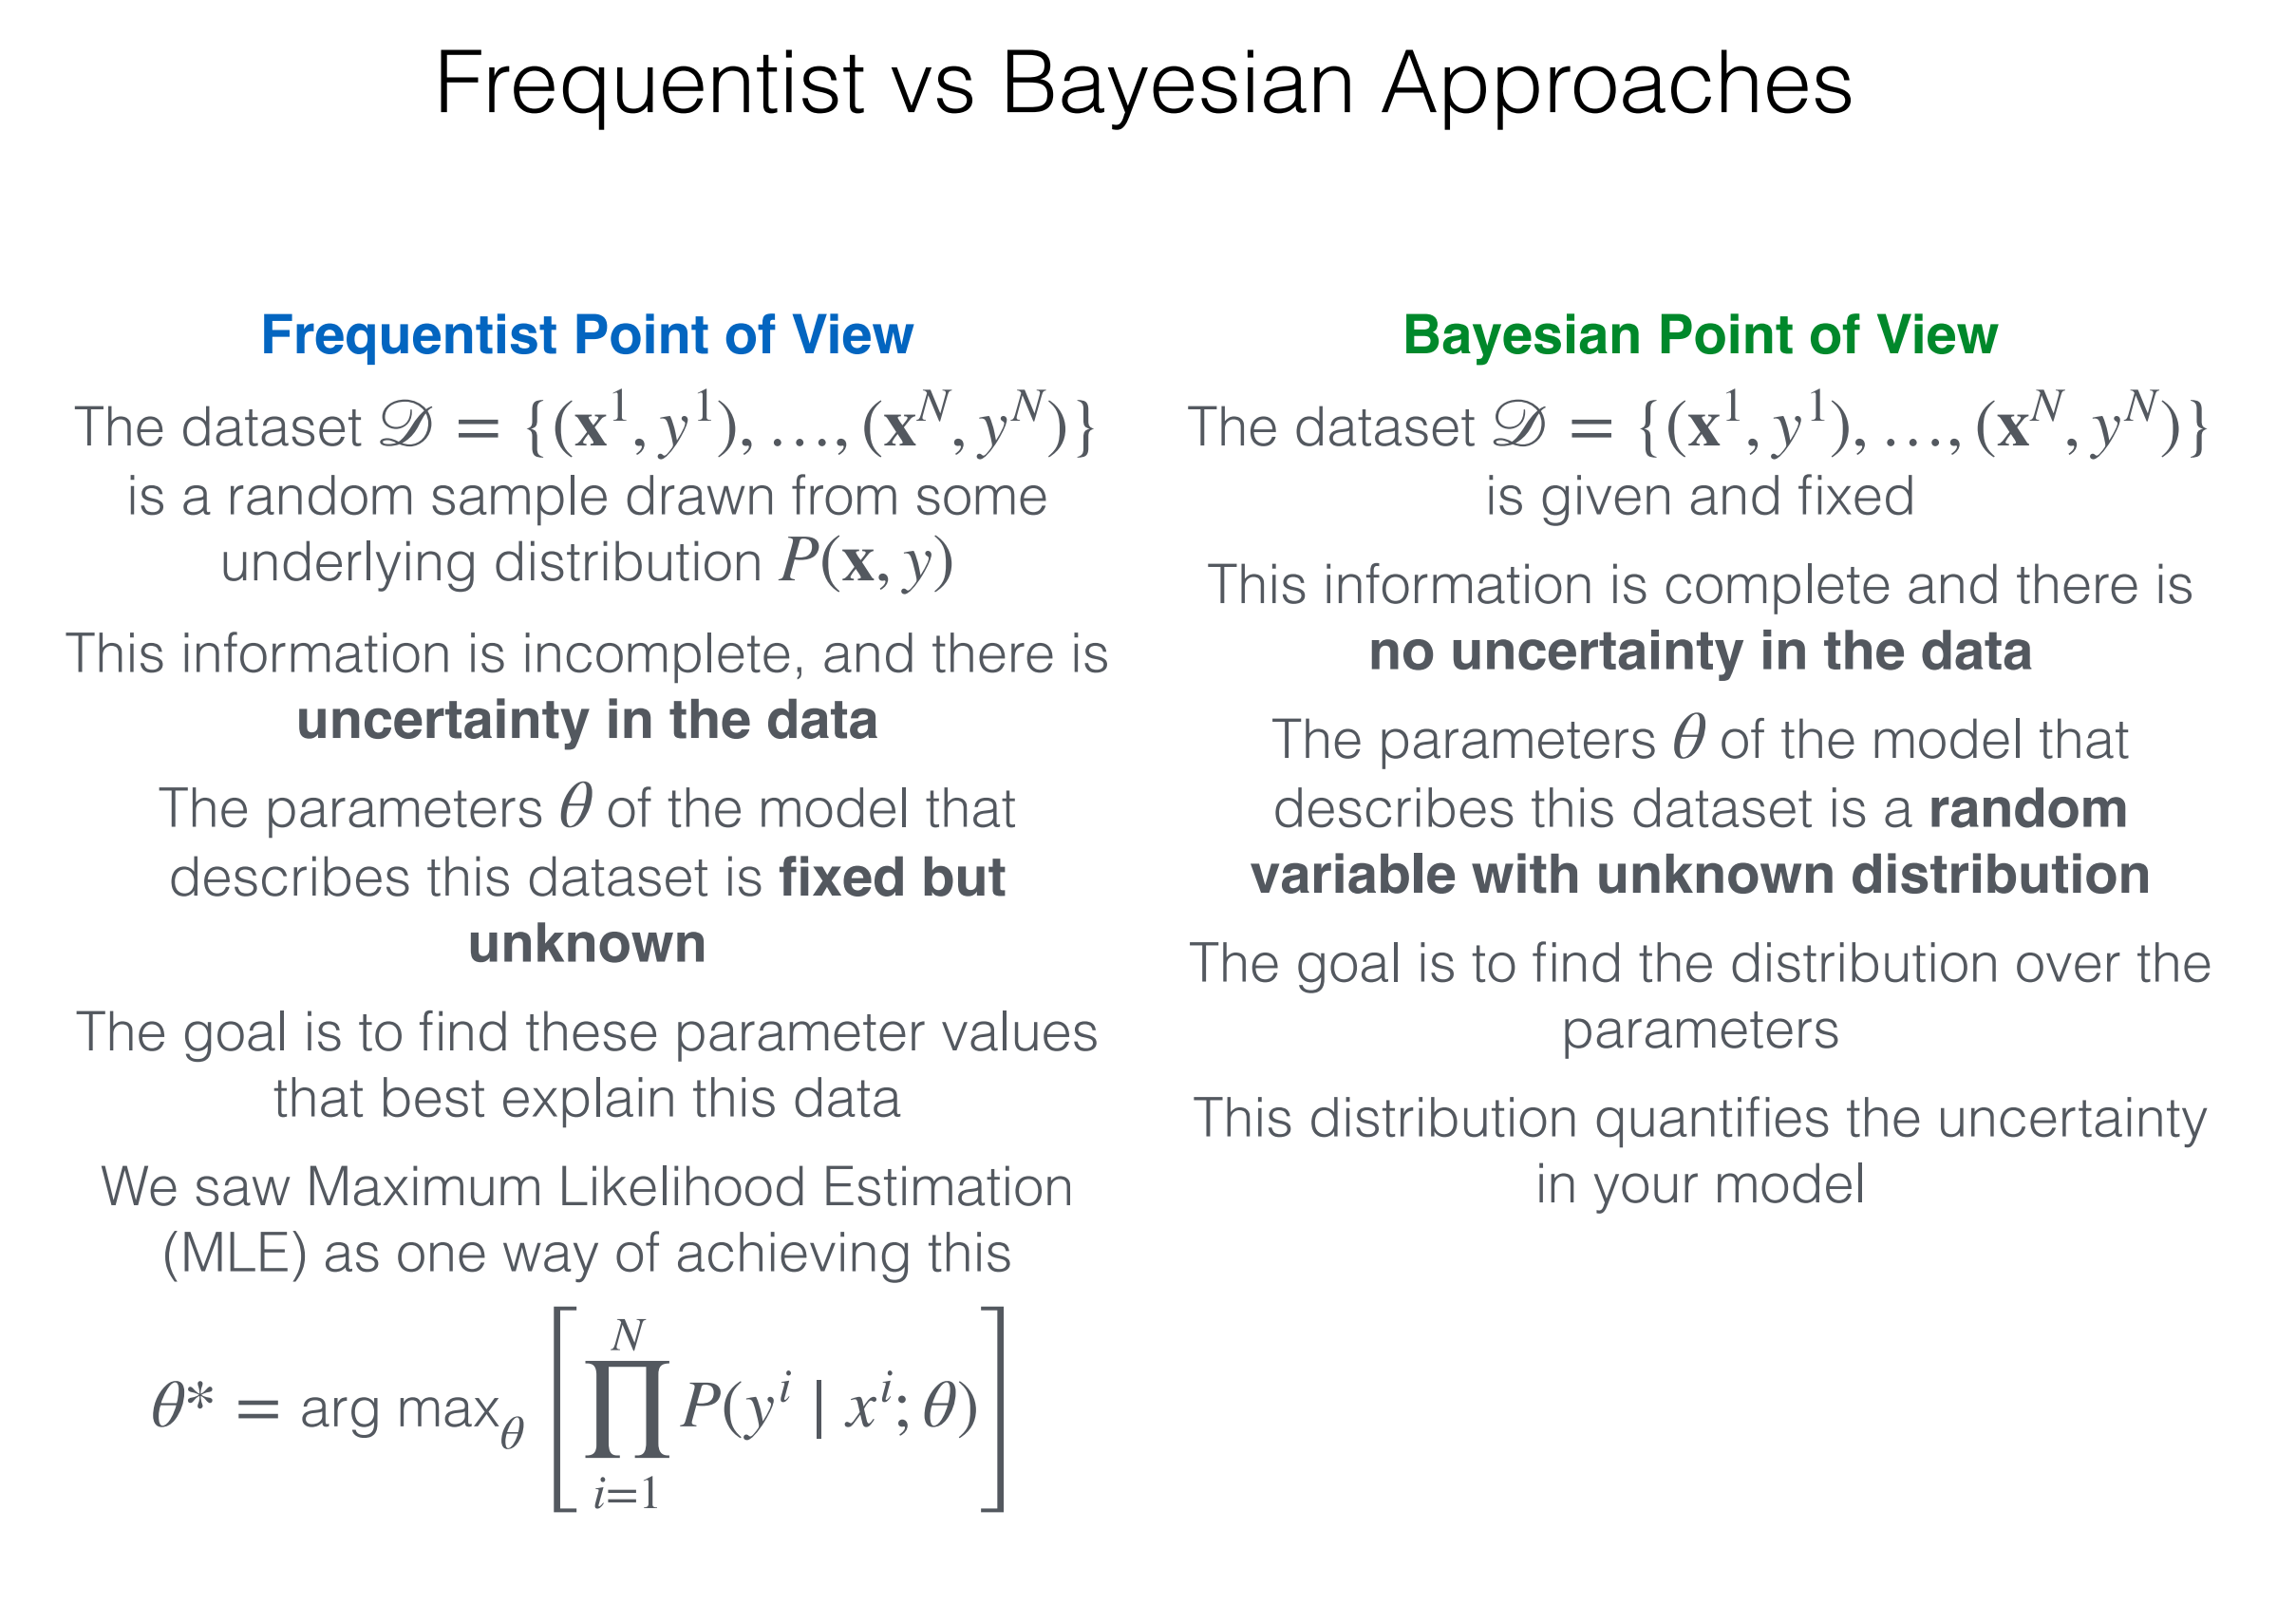
\includegraphics[width=16cm]{6.1.5_Comparison.png}
\end{figure}

\subsubsection{Summary}
In summary, Bayesian decision theory provides a method to make decisions by combining probability and utility. It can be applied in various fields, from medicine to finance to machine learning.
\newpage

\subsection{Bayesian Parameter Estimation}
Let us start with some prior distribution $P(\theta)$, which encodes our knowledge about the parameters before looking at the data. And we are given a dataset $\mathcal{D} = \{ (\bm{x}^1, y^1), (\bm{x}^2, y^2), ..., (\bm{x}^N, y^N) \}$. Our goal is to find out the posterior distribution of $\theta$ given the dataset $\mathcal{D}$: $P(\theta \mid \mathcal{D})$. We will use the Bayes Theorem.
\begin{align*}
    P(\theta \mid \mathcal{D})
    &= \frac{P(\mathcal{D} \mid \theta)P(\theta)}{P(\mathcal{D})}\\
    &= \frac{P(\mathcal{D} \mid \theta)P(\theta)}{\int_{\theta} P(\mathcal{D} \mid \theta)P(\theta)d\theta}\\
    &= \frac{ \left[ \prod_{i=1}^{N}P( y^i \mid \bm{x}^i ,\theta) \right] P(\theta)}{\int_{\theta} \left[ \prod_{i=1}^{N}P( y^i \mid \bm{x}^i ,\theta) \right]P(\theta)d\theta}
\end{align*}
Here is an example: Suppose we are going to estimate the parameter of a biased coin. We flipped 100 time and we get heads for 55 time and tail for 45 times. What would be the probability that it will be heap for the next flip? Flipping the coin can be seen as independent Bernoulli random variables with parameter $\theta$:
\[ p(\theta \mid \mathcal{D}) \propto p(\mathcal{D} \mid \theta)p(\theta) \]
Then under the Bernoulli model with i.i.d observations, we have the following:
\begin{align*}
    \text{Likelihood: } p(\mathcal{D} \mid \theta) &= \theta^{N_H}(1-\theta)^{N_T}\\
    \text{Choose a prior: } p(\theta; a,b) &= \frac{\Gamma(a+b)}{\Gamma(a)\Gamma(b)}\theta^{a-1}(1-\theta)^{b-1}\\
    & \propto \theta^{a-1}(1-\theta)^{b-1}\\
    p(\theta \mid \mathcal{D}) & \propto p(\mathcal{D} \mid \theta)p(\theta)\\
    & \propto \left[ \theta^{N_H}(1-\theta)^{N_T} \right] \left[ \theta^{a-1}(1-\theta)^{b-1} \right]\\
    & = \theta^{N_H+a-1}(1-\theta)^{N_T+b-1}
\end{align*}
After calculation, we can also find out the expectation:\\
 \\
Given the posterior distribution parameters \( a = 56 \) and \( b = 46 \), the expected value of \( \theta \) is given by:
\[ \mathbb{E}[\theta] = \frac{a}{a+b} \]
Substituting in the values:
\[ \mathbb{E}[\theta] = \frac{56}{56+46} = \frac{56}{102} = \frac{28}{51} \]
Thus, the best estimate for the probability of getting heads on the next flip, based on the observed data and the chosen prior, is \( \frac{28}{51} \) or approximately \( 0.549 \).
\subsubsection{Gamma Function and Beta Distribution*}
\textbf{1. Gamma Function (\( \Gamma \)): }\\
The Gamma function is a mathematical function that generalizes the factorial function to non-integer values. It's defined as:
\[ \Gamma(z) = \int_0^\infty t^{z-1} e^{-t} \, dt \]
for complex numbers \( z \) with a positive real part.
Some key properties and facts about the Gamma function:
\begin{itemize}
  \item For positive integers \( n \):
  \[ \Gamma(n) = (n-1)! \]
  This shows how the Gamma function generalizes the factorial function.
  
  \item The Gamma function is defined for all complex numbers except non-positive integers (where it has poles).
\end{itemize}
\textbf{2. Beta Distribution: }\\
The Beta distribution is a continuous probability distribution defined on the interval [0, 1]. It's commonly used in Bayesian statistics to model the distribution of random variables that represent probabilities.
The probability density function (pdf) of the Beta distribution is:
\[ f(x; a, b) = \frac{x^{a-1} (1-x)^{b-1}}{B(a,b)} \]
where \( 0 \leq x \leq 1 \) and \( a, b > 0 \). The function \( B(a,b) \) is the Beta function, which serves as a normalization constant to ensure that the total probability integrates to 1.
The **Beta function** is defined in terms of the Gamma function:
\[ B(a,b) = \frac{\Gamma(a) \Gamma(b)}{\Gamma(a+b)} \]
Some properties of the Beta distribution:
\begin{itemize}
  \item The \textbf{mean} of the Beta distribution is:
  \[ \mu = \frac{a}{a+b} \]
  
  \item The \textbf{variance} is:
  \[ \sigma^2 = \frac{ab}{(a+b)^2(a+b+1)} \]

  \item The shape of the Beta distribution is determined by the parameters \( a \) and \( b \):
  \begin{itemize}
    \item If \( a = b = 1 \), it's the uniform distribution on [0,1].
    \item If \( a > b \), the distribution is skewed towards 1.
    \item If \( a < b \), the distribution is skewed towards 0.
    \item If \( a = b > 1 \), the distribution is symmetric and bell-shaped.
  \end{itemize}
\end{itemize}
The Beta distribution is particularly useful in Bayesian statistics because it's the conjugate prior for the Bernoulli, binomial, and negative binomial likelihoods. This means that if you start with a Beta prior and observe data that follows one of these likelihoods, the posterior distribution will also be a Beta distribution.

\subsection{Prediction with Bayesian Models}
Given the training set \( \mathcal{D}\) and a new observation set \( \mathcal{D'}\), posterior predictive distribution is the distribution over future observables given the past observations. We can compute it by marginalizing out the parameters. Here are the steps:
\begin{align*}
    p(\mathcal{D'} \mid \mathcal{D}) &= \int p(\theta \mid \mathcal{D})p(\mathcal{D'} \mid \theta ) d\theta\\
    \theta_{pred} &= Pr(x'=H \mid \mathcal{D})\\
    &= \int p(\theta \mid \mathcal{D})Pr(x'=H \mid \mathcal{D})d\theta\\
    &= \int Beta(\theta; N_H+a, N_T+b) \cdot \theta d\theta\\
    &= \mathbb{E}_{Beta}(\theta; N_H+a, N_T+b)\\
    &= \frac{N_H+a}{N_H+N_T+a+b}
\end{align*}
Let's break down the above steps.
\begin{enumerate}
    \item \textbf{Marginalizing Out the Parameters}\\
    \[ p(\mathcal{D'} \mid \mathcal{D}) = \int p(\theta \mid \mathcal{D})p(\mathcal{D'} \mid \theta ) d\theta \]
This equation represents the probability of observing the new data \( \mathcal{D'} \) given the training data \( \mathcal{D} \). We compute this by integrating (or averaging) over all possible values of the parameter \( \theta \). The term \( p(\theta \mid \mathcal{D}) \) is the posterior distribution of \( \theta \) given the training data, and \( p(\mathcal{D'} \mid \theta ) \) is the likelihood of the new data given \( \theta \).
    \item \textbf{Predictive Probability for a Single New Observation}\\
    \[ \theta_{pred} = Pr(x'=H \mid \mathcal{D}) \]
This represents the probability that a single new observation \( x' \) is a head (H) given the training data \( \mathcal{D} \).
    \item \textbf{Computing the Predictive Probability}\\
    \[ \theta_{pred} = \int p(\theta \mid \mathcal{D})Pr(x'=H \mid \theta)d\theta \]
Here, we're averaging the probability of observing a head over all possible values of \( \theta \), weighted by the posterior distribution of \( \theta \).
    \item \textbf{Substituting the Posterior Distribution}\\
    \[ \theta_{pred} = \int Beta(\theta; N_H+a, N_T+b) \cdot \theta d\theta \]
Given that the posterior distribution of \( \theta \) is a Beta distribution with parameters \( N_H+a \) and \( N_T+b \) (where \( N_H \) is the number of observed heads and \( N_T \) is the number of observed tails), we multiply this by \( \theta \) (the probability of observing a head) and integrate.
    \item \textbf{Expectation of the Beta Distribution}\\
    \[ \theta_{pred} = \mathbb{E}_{Beta}(\theta; N_H+a, N_T+b) \]
The integral in the previous step is essentially computing the expected value (or mean) of \( \theta \) under the Beta distribution.
    \item \textbf{Computing the Expectation}\\
    \[ \theta_{pred} = \frac{N_H+a}{N_H+N_T+a+b} \]
The expected value of the Beta distribution is given by \( \frac{a}{a+b} \). Substituting in the values for \( a \) and \( b \) from the posterior distribution, we get the above equation.
\end{enumerate}
In summary, the provided equations describe how to compute the probability of observing a particular outcome (like a head in a coin flip) for new data based on previously observed data, by averaging over all possible values of the underlying parameter \( \theta \) in a Bayesian framework. The result is a predictive distribution that takes into account both the observed data and our prior beliefs about \( \theta \). \\
 \\
 Now let's generalize what we just got. Suppose we are given the training set \( \mathcal{D}\)and a new observation \(\bm{x}\), what is the value of y? What we are looking for is the distribution \(P(y \mid \bm{x},\mathcal{D})\).\\ 
 1. For logistic regression:
 \[P(y \mid \bm{x},\theta)=h_{\theta}(\bm{x})=\frac{1}{1+e^{-\theta^{T}\bm{x}}} \]
 2. We also have:
 \[ P(\theta \mid \mathcal{D}) = \frac{ \left[ \prod_{i=1}^{N}P( y^i \mid \bm{x}^i ,\theta) \right] P(\theta)}{\int_{\theta} \left[ \prod_{i=1}^{N}P( y^i \mid \bm{x}^i ,\theta) \right]P(\theta)d\theta}\]
 3. We combine them together:
 \[ P(y \mid \bm{x},\mathcal{D}) = \int_{\theta} P(y \mid \bm{x},\theta)P(\theta \mid \mathcal{D}) d\theta = \int_{\theta} h_{\theta}(\bm{x})P(\theta \mid \mathcal{D}) d\theta \]
 But it is a hard-to-compute integral.
 \subsection{Bayesian Model in Practise}
In practice we normally have two options:
\begin{itemize}
    \item \textbf{Option 1: }Do away with the full integral to integrate across the entire parameter distribution. Instead we follow the steps:
    \begin{enumerate}
        \item Compute the point estimate of the parameters:
        \[ \theta_{\text{MAP}} = \arg \max_\theta \prod_{i=1}^{N}P(y^i \mid \bm{x}^i, \theta) \cdot P(\theta)\]
        \item Use the estimate to compute $y$ for a new $\bm{x}$ (Inference)
        \[ \hat{y} = \arg \max_y p(y \mid \bm{x}; \theta = \theta_{\text{MAP}})\]
        \item This is called \textbf{Maximum A Posterior (MAP)} estimate. It is very similar to the Maximum Likelihood Estimate (MLE) but with an additional prior term.
    \end{enumerate}
    \item \textbf{Option 2:} Choose the distribution function $P(y \mid \bm{x},\theta)$ such that the integral can be computed analytically.
\end{itemize}

\subsection{Bayesian Linear Regression}

Bayesian linear regression combines the principles of linear regression with Bayesian inference to estimate the parameters of a linear model.

\subsubsection{Three Key Steps in Bayesian Methods}

\begin{enumerate}
    \item \textbf{Prior Distribution}: \\Represents our initial beliefs about the parameters before observing any data.
    \item \textbf{Likelihood}: \\Describes the probability of observing the data given the model parameters.
    \item \textbf{Posterior Distribution}: \\Combines the prior and the likelihood to give an updated belief about the parameters after observing the data.
\end{enumerate}

\subsubsection{Prior Distribution}
The prior distribution, \( p(w) \), describes our beliefs about the weights \( w \) before observing any data. A common choice is a Gaussian prior for \( w \):

\[
w \sim \mathcal{N}(m_0, S_0)
\]
Where:
\begin{itemize}
    \item \( m_0 \) is the prior mean, often set to a zero vector.
    \item \( S_0 \) is the prior covariance matrix, describing the uncertainty in the weights.
\end{itemize}

\subsubsection{Likelihood}
The likelihood function describes the probability of observing the data given the model parameters. In linear regression, it's commonly assumed that the errors are independent and identically distributed with Gaussian noise:

\[
y_i \sim \mathcal{N}(w^T x_i, \sigma^2)
\]
For the entire dataset \( \mathcal{D} \):

\[
p(\mathcal{D} | w) = \prod_{i=1}^N \mathcal{N}(y_i; w^T x_i, \sigma^2)
\]

\subsubsection{Posterior Distribution}
The posterior distribution combines the prior and the likelihood to give an updated belief about the parameters:

\[
p(w | \mathcal{D}) = \frac{p(\mathcal{D} | w) p(w)}{p(\mathcal{D})}
\]
Where:
\begin{itemize}
    \item \( p(w | \mathcal{D}) \) is the posterior distribution.
    \item \( p(\mathcal{D} | w) \) is the likelihood.
    \item \( p(w) \) is the prior distribution.
    \item \( p(\mathcal{D}) \) is the marginal probability of the data, also known as the normalization constant.
\end{itemize}
When using a Gaussian prior and Gaussian likelihood, the posterior distribution is also Gaussian, simplifying computation and inference.

\subsubsection{How to Choose the Prior}
Prior should reflect your knowledge about the distribution before looking at the data.
\begin{itemize}
    \item \textbf{Objective Priors: }should maximize the impact of data on posterior. Non-Informative Priors are a type of objective priors (e.g., uniform distribution)
    \item \textbf{Subjective Priors: } that capture some domain/external knowledge about the problem (e.g., Gaussian priors)
    \item \textbf{Conjugate Priors: }a prior is considered conjugate with respect to the likelihood if the resulting posterior distribution is of the same form as the prior distribution — used primarily for simplifying the calculation of the integral
\end{itemize}

\subsubsection{Maths for Bayesian Linear Regression}
TO BE COMPLETED


\newpage
\section{Probabilistic Models}
\subsection{Linear Regression Model}


\newpage
\section{Support Vector Machine}
Suppose we are given a bunch of data points that are not labeled, how do we find a separator that can best divide them into 2 classes? This process is similar to find a hyperplane (which it is). One way to do it is the Perceptron Learning Algorithm. But is there a better way to strengthen the line's power? The answer is to apply Support Vector Machine.\\
 \\
To find the best plane is the mission of SVM. That is to say, we use SVM to find a separating hyperplane that has the largest margin. This intuitive idea is backed by clear theory and it usually works in really/application.\\
 \\
 There are three keys in Support Vector Machine:
 \begin{enumerate}
     \item Seeks a large margin separator to improve generalization;
     \item Uses optimization theory to find an optimal solution (with few errors) efficiently;
     \item Uses kernel tricks to make computations efficient in cases where the feature vectors are huge.
 \end{enumerate}
Mathematically, the SVM model can be expressed as follows:

\subsection{Linear SVM}
Assume we have a binary classification task with a training dataset \( \{(x_i, y_i)\} \), where \( x_i \) are feature vectors and \( y_i \) are class labels for each \( x_i \), which can be 1 or -1. SVM tries to find a separating hyperplane \( w \cdot x + b = 0 \), where \( w \) is the normal vector, and \( b \) is the bias term. The choice of this hyperplane is based on maximizing the margin:
\[ \text{margin} = \frac{2}{\|w\|} \]
In this optimization problem, we maximize the margin while ensuring all data points are correctly classified, that is for all \( i \):
\[ y_i (w \cdot x_i + b) \geq 1 \]

\subsection{Soft Margin SVM}
When the data is not linearly separable, we allow some data points to be on the wrong side. Slack variables \( \xi_i \) are introduced to measure the degree of misclassification of each point. The optimization problem becomes:
\[ \min_{w,b,\xi} \frac{1}{2} \|w\|^2 + C \sum_{i=1}^{n} \xi_i \]
\[ \text{subject to } y_i (w \cdot x_i + b) \geq 1 - \xi_i \text{ and } \xi_i \geq 0 \text{ for all } i \]
Here \( C \) is a regularization parameter, controlling the trade-off between margin size and classification error.

\subsection{Kernel Trick}
For non-linearly separable data, SVMs can use a technique known as the kernel trick to implicitly map the input space into a higher-dimensional feature space where the data may be linearly separable. Commonly used kernel functions include polynomial, radial basis function (RBF, also known as Gaussian), and sigmoid kernels.\\
 \\
With the kernel function, the decision rule becomes:
\[ f(x) = \text{sign} \left( \sum_{i=1}^{n} \alpha_i y_i K(x_i, x) + b \right) \]
where \( \alpha_i \) are Lagrange multipliers, which are solutions to the dual problem of the SVM, and \( K(x_i, x) \) is the kernel function, computing the similarity between the input feature vector \( x \) and the training sample \( x_i \).\\
 \\
During the training phase, the objective of SVM is to determine the parameters of the separating hyperplane \( w \) and \( b \), and for kernel SVM, to determine the Lagrange multipliers \( \alpha_i \). This is typically done by solving a dual problem that can be transformed into a quadratic programming problem, and then using specialized algorithms such as Sequential Minimal Optimization (SMO).\\
 \\
Once trained, the model can be used to predict the class of new data points. If a data point lies on one side of the hyperplane, it is classified into the positive class; if it is on the other side, it is classified into the negative class. For kernel SVMs, the classification decision is based on the computation of similarity between the kernel function and the support vectors.


\newpage
\section{Neural Networks}



\newpage
\section{Deep Learning}



\newpage
\section{CONTINUED}







\end{document}